\documentclass[oneside,12pt]{book}
\usepackage[utf8]{inputenc}
\usepackage{standalone}
\usepackage[margin=2.5cm]{geometry}
\usepackage{graphicx}
\usepackage{hyperref}
\usepackage{lmodern}
\usepackage{float}
\usepackage[spanish]{babel}
\usepackage{csquotes}
\usepackage[figurename=Ilustración]{caption}
\usepackage[numbers]{natbib}
\usepackage{ragged2e}
\usepackage{array}
\usepackage{multirow}
\usepackage{parskip}
\usepackage{listings}
\usepackage{epigraph}
\usepackage{lipsum} % Texto de relleno en plantilla
% \usepackage{svg} % Ya no se usa, convertido a pdf directos

\usepackage{algorithm}
\usepackage{algpseudocode}
\usepackage{filecontents} % Para incluir la bibliografía en este mismo archivo

% --- BIBLIOGRAFÍA ---
\begin{filecontents}{ref.bib}
@misc{disecan2026,
  author = {IATEXT ULPGC},
  title = {Buscador Textual DiSeCan del Parlamento de Canarias},
  year = {2026},
  url = {https://iatext.ulpgc.es/es/aplicaciones/buscador-textual}
}

@article{robertson2009probabilistic,
  title={The probabilistic relevance framework: BM25 and beyond},
  author={Robertson, Stephen and Zaragoza, Hugo and others},
  journal={Foundations and Trends{\textregistered} in Information Retrieval},
  volume={3},
  number={4},
  pages={333--389},
  year={2009},
  publisher={Now Publishers, Inc.}
}

@inproceedings{cormack2009reciprocal,
  title={Reciprocal rank fusion outperforms condorcet and individual rank learning methods},
  author={Cormack, Gordon V and Clarke, Charles LA and Buettcher, Stefan},
  booktitle={Proceedings of the 32nd international ACM SIGIR conference on Research and development in information retrieval},
  pages={758--759},
  year={2009}
}

@misc{chromadb2025,
  author = {Chroma Inc.},
  title = {Chroma: The AI-native open-source vector database},
  year = {2025},
  url = {https://www.trychroma.com/}
}

@article{wang2022text,
  title={Text embeddings by weakly-supervised contrastive pre-training},
  author={Wang, Liang and Yang, Nan and Huang, Xiaolong and Jiao, Binxing and Ding, Linjun and Jiang, Daxin and Yan, Rui and Wei, Furu},
  journal={arXiv preprint arXiv:2212.03533},
  year={2022}
}

@article{bonifacio2021mmarco,
  title={mMARCO: A multilingual version of the MS MARCO passage ranking dataset},
  author={Bonifacio, Luiz and Jeronymo, Vitor and Ribeiro, Hugo Queiroz and Lotufo, Roberto and Nogueira, Rodrigo},
  journal={arXiv preprint arXiv:2108.13897},
  year={2021}
}
\end{filecontents}
% --------------------

% Glosario de términos - BEGIN
\usepackage{glossaries}

\makeglossaries

\newglossaryentry{rag}
{
    name=RAG,
    description={Retrieval-Augmented Generation. Arquitectura que mejora las respuestas de un modelo de lenguaje apoyándose en bases de datos externas}
}

\newglossaryentry{vllm}
{
    name=vLLM,
    description={Servidor de inferencia de alta eficiencia para Modelos de Lenguaje de Gran Escala}
}

\newacronym{iatext}{IATEXT}{Instituto Universitario de Análisis y Aplicaciones Textuales}

\newacronym{disecan}{DiSeCan}{Buscador de los Diarios de Sesiones de Canarias}

\newacronym{iagen}{IAGen}{Inteligencia Artificial Generativa}

\newacronym{llm}{LLM}{Large Language Model (Gran Modelo de Lenguaje)}

\newacronym{sql}{SQL}{Structured Query Language}

\newacronym{ods}{ODS}{Objetivos de Desarrollo Sostenible}

\newacronym{crisp-dm}{CRISP-DM}{Cross-Industry Standard Process for Data Mining}

\newglossaryentry{bm25}
{
    name=BM25,
    description={Best Matching 25. Algoritmo de recuperación de información basado en term frequency-inverse document frequency (TF-IDF)}
}

\newglossaryentry{rrf}
{
    name=RRF,
    description={Reciprocal Rank Fusion. Técnica empírica que combina los resultados de la búsqueda léxica y semántica para generar un ranking unificado de mayor calidad}
}

\newglossaryentry{crossencoder}
{
    name=Cross-Encoder,
    description={Arquitectura basada en Transformers que procesa simultáneamente una consulta y un documento para predecir con alta precisión su grado de relevancia}
}

\newglossaryentry{chromadb}
{
    name=ChromaDB,
    description={Base de datos vectorial \textit{open-source} empleada para el almacenamiento y búsqueda semántica de \textit{embeddings}}
}

% Glosario de términos - END

%\usepackage{fancyhdr}
\usepackage{color}
\usepackage{graphicx,xcolor}

\renewcommand{\lstlistingname}{Algoritmo}
\floatname{algorithm}{Algoritmo}
\renewcommand{\listalgorithmname}{Índice de~\lstlistingname s}

\lstset{
        basicstyle=\fontsize{7}{11}\ttfamily,
        language=Python,
        captionpos=b,
}

\usepackage{titlesec}
\setcounter{secnumdepth}{3}
\titleformat{\chapter}[display]
{\normalfont\huge\bfseries}{\chaptertitlename\ \thechapter}{20pt}{\Huge}

\urlstyle{same}
\title{Implementación de un sistema de consulta con Inteligencia Artificial sobre un gran
número de documentos}
\author{David Suárez Martel}
\date{Curso 2025 - 2026}
\renewcommand{\contentsname}{Contenido}
\renewcommand{\figurename}{}
\usepackage{pifont}
\renewcommand\labelitemi{\ding{52}}

\begin{document}

\begin{titlepage}

\begin{center}

\vspace*{0.25in}
\begin{figure}[htb]
\begin{center}

\includegraphics[width=15cm]{Ilustraciones/NuevoLogoEII.png}
%
\includegraphics[width=15cm]{Ilustraciones/LogoEII.jpg}
%
\includegraphics[width=20cm]{Ilustraciones/Logo_EII+ULPGC.png}
\end{center}
\end{figure}

\vspace*{0.25in}
\vspace*{0.25in}
\begin{Huge}
    \textbf{Trabajo de Fin de Grado} \\
\end{Huge}
\vspace*{0.5in}

\noindent\hfil\rule{17cm}{0.2mm}\hfil\\

\vspace*{0.1in}
\begin{Huge}
    \textbf{Implementación de un sistema de consulta con Inteligencia Artificial sobre un gran
número de documentos} \\
\end{Huge}
\vspace*{0.3in}
\begin{large}
TITULACIÓN: Grado en Ingeniería Informática \\
\vspace*{0.1in}
AUTOR: David Suárez Martel \\
\end{large}
\vspace*{0.3in}
\noindent\hfil\rule{17cm}{0.2mm}\hfil\\
\vspace*{0.1in}
\begin{large}
TUTORIZADO POR: \\
Francisco Javier Carreras Riudavets \\
\end{large}
\vspace*{0.3in}
Fecha [Junio/2026]

\end{center}


\end{titlepage}


\input{TFT04C.tex}

\newpage
\pagenumbering{roman}

\input{Agradecimientos.tex}

\clearpage
{\setlength{\parskip}{8mm}
{\huge{\textbf{Resumen}}}

Los Diarios de Sesiones del Parlamento de Canarias son una fuente documental crítica para la preservación de la memoria democrática. El presente Trabajo de Fin de Grado propone el diseño y desarrollo de una arquitectura de Generación Aumentada por Recuperación (RAG) de naturaleza híbrida para modernizar la herramienta de búsqueda actual (DiSeCan). Integrando bases de datos relacionales (SQL) con bases de datos vectoriales, el sistema permite superar las limitaciones de la búsqueda por palabras clave, ofreciendo consultas semánticas en lenguaje natural apoyadas en metadatos. La implementación se diseña para un entorno cerrado, garantizando la soberanía de los datos y la mitigación de alucinaciones.

\newpage

{\huge{\textbf{Abstract}}}

   The Congressional Record of the Parliament of the Canary Islands becomes critical for the preservation of democratic memory. This Bachelor's Thesis proposes the design and development of a hybrid Retrieval Augmented Generation (RAG) architecture to modernize the current search tool (DiSeCan). By integrating relational databases (SQL) with vector databases, the system overcomes the limitations of keyword searches, offering semantic queries in natural language supported by metadata. The implementation is designed for an on-premises environment, guaranteeing data sovereignty and mitigating data hallucinations.

}
\tableofcontents

\listofalgorithms 

\listoffigures

\listoftables


\clearpage
\pagenumbering{arabic}

\chapter{Introducción}
En este capítulo se expone el \textbf{contexto} general del trabajo, los conceptos tecnológicos indispensables que motivan a su desarrollo y, finalmente, la estructura en la que se organiza el resto del documento.

\section{Contexto y motivación}
La preservación de la memoria parlamentaria y la transparencia en la gestión pública por parte de los representantes se encuentran principalmente en los Diarios de Sesiones del Parlamento de Canarias, convirtiéndolos en una valiosa fuente documental. Durante décadas, estas actas han registrado las intervenciones, debates y acuerdos legislativos del archipiélago. Actualmente, el acceso y la consulta a este gran conjunto de ficheros son facilitados por el \gls{iatext} \cite{iatext_web} a través de herramientas de recuperación especializadas como el buscador textual \textbf{\gls{disecan}}.

No obstante, la evolución tecnológica y las crecientes necesidades de investigadores y ciudadanos demandan sistemas de recuperación de información más intuitivos y precisos disponibles para el público. Los buscadores tradicionales, basados puramente en coincidencias \textit{booleanas} o expresiones regulares (\textit{Regex}), presentan ciertas limitaciones al no ser capaces de comprender ni el contexto semántico ni la intención detrás del mensaje que presenta el usuario. Esta limitación es el principal motivo para el desarrollo de este trabajo, cuyo propósito es investigar e implementar arquitecturas modernas basadas en \gls{iagen} para conseguir una versión del sistema de búsqueda más contextual y eficaz.

\section{Conceptos básicos: Hacia el RAG Híbrido}
Para superar los inconvenientes de los buscadores tradicionales, este proyecto se basa en la arquitectura de Generación Aumentada por Recuperación (\gls{rag}) \cite{lewis2020rag}. Esta técnica permite a los \gls{llm} generar respuestas precisas consultando bases de datos específicas y cerradas como fuentes de verdad, mitigando así el riesgo de generar información falsa o \textit{alucinaciones} \cite{ji2023hallucination}.


Concretamente, se propone el diseño de un sistema \textbf{\gls{rag} Híbrido}. Esta solución integra la precisión de las bases de datos relacionales (\gls{sql}), ideales para filtrar por metadatos institucionales (como el nombre del orador, la fecha o la legislatura), con la flexibilidad que ofrecen las bases de datos vectoriales, capaces de realizar búsquedas por similitud semántica. Todo ello siendo ejecutado en una infraestructura local para garantizar la \textbf{soberanía, seguridad y privacidad} de los datos utilizados.

Como resultado, este trabajo aporta un prototipo funcional de asistente conversacional para el \gls{disecan}, compuesto por un motor de búsqueda híbrido y una interfaz web interactiva diseñada para la comodidad y usabilidad por parte del usuario final.

\section{Organización del documento}
El resto del documento está integrado por los siguientes capítulos, estructurados conforme a las directrices de la Escuela de Ingeniería Informática:

\begin{itemize}
    \item El \textbf{Capítulo 2} expone el estado actual del problema, los antecedentes tecnológicos y los objetivos específicos planteados inicialmente para el desarrollo del trabajo.
    \item El \textbf{Capítulo 3} detalla las aportaciones del proyecto, la justificación de las competencias adquiridas durante el grado y el alineamiento con los \gls{ods}.
    \item El \textbf{Capítulo 4} describe la metodología aplicada (\gls{crisp-dm}) y las fases técnicas de diseño, desarrollo e implementación de la arquitectura híbrida.
    \item El \textbf{Capítulo 5} presenta los resultados obtenidos tras la experimentación, validación y despliegue del sistema propuesto.
    \item El \textbf{Capítulo 6} recoge las conclusiones derivadas del proyecto, evaluando la consecución de objetivos, y propone posibles líneas de trabajo futuro.
    \item Finalmente, el \textbf{Capítulo 7} incluye consideraciones adicionales como el marco normativo y la legislación aplicable a los sistemas de Inteligencia Artificial en el sector público.
\end{itemize}

\chapter{Estado actual y objetivos iniciales}
%\input{EstadoDelArte.tex}
% REVISADO HASTA AQUÍ
\section{Motivación y antecedentes}
Actualmente, el corpus del Parlamento de Canarias supera las 71.000 páginas de transcripciones. La recuperación tradicional presenta desafíos técnicos, ya que la búsqueda de términos aislados ignora a menudo la intención semántica del usuario. Surge así la necesidad de sistemas que combinen la precisión de los filtros SQL (por diputado, fecha o legislatura) con la comprensión conceptual de los vectores de alta dimensionalidad.

\section{Objetivos}
En la propuesta inicial del TFT se plantearon los siguientes objetivos principales:
\begin{itemize}
    \item \textbf{Implementación de Búsqueda Híbrida:} Integrar técnicas de recuperación relacional (SQL) con recuperación semántica vectorial.
    \item \textbf{Estructuración mediante Metadatos:} Diseñar un chunking consciente del contexto que evite la fragmentación arbitraria de las intervenciones.
    \item \textbf{Despliegue On-Premise:} Configurar un entorno local eficiente mediante contenedores y \gls{vllm} para ejecutar modelos de lenguaje a gran escala sin comprometer la privacidad institucional.
\end{itemize}

\chapter{Aportaciones del trabajo}
\chaptermark{Competencias, aportaciones y ODS}
%\input{Competencias.tex}

\section{Principales aportaciones}
Este TFT aporta al entorno socio-económico canario una herramienta de vanguardia para la democratización de la información legislativa. A nivel técnico, demuestra la viabilidad de implementar arquitecturas Context-Aware RAG en infraestructuras locales del IATEXT, mitigando las alucinaciones de los modelos genéricos mediante el anclaje estricto en fuentes oficiales.

\section{Competencias específicas}
Este trabajo cubre de forma directa las siguientes competencias específicas del Grado en Ingeniería Informática:
\begin{itemize}
    \item \textbf{CI15:} Conocimiento y aplicación de los principios fundamentales y técnicas básicas de los sistemas inteligentes. Se cubre mediante la orquestación del motor LLM y la búsqueda semántica vectorial.
    \item \textbf{CI13:} Herramientas para el almacenamiento, procesamiento y acceso a sistemas de información. Cubierto a través de la integración de bases de datos relacionales (SQL) y su estructuración para el sistema RAG.
    \item \textbf{CI7:} Conocimiento y utilización eficiente de tipos y estructuras de datos. Evidenciado en la lógica de indexación híbrida y chunking por metadatos.
\end{itemize}

\section{Alineamiento con los objetivos de desarrollo sostenible}

\begin{table}[!htbp]
\caption{Grado de relación del TFT con los objetivos de desarrollo sostenible.}
\label{tab:ODS}
\centering
\begin{tabular}{|l|c|c|c|c|}
\cline{1-5}
  & \multicolumn{4}{c|}{Grado de relación} \\ \cline{2-5} 
 ODS & 0 & 1 & 2 & 3 \\
  & No procede & Bajo & Medio & Alto \\  
  \cline{1-5} 
1 Fin de la Pobreza & X & & & \\ \cline{1-5}
2 Hambre cero & X & & & \\ \cline{1-5}
3 Salud y Bienestar & X & & & \\ \cline{1-5}
4 Educación de calidad & & X & & \\ \cline{1-5}
5 Igualdad de género & X & & & \\ \cline{1-5}
6 Agua limpia y saneamiento & X & & & \\ \cline{1-5}
7 Energía Asequible y no contaminante & X & & & \\ \cline{1-5}
8 Trabajo decente y crecimiento económico & X & & & \\ \cline{1-5}
9 Industria, Innovación e Infraestructuras & & & & X \\ \cline{1-5}
10 Reducción de las desigualdades & X & & & \\ \cline{1-5}
11 Ciudades y comunidades sostenibles & X & & & \\ \cline{1-5}
12 Producción y consumo sostenibles & X & & & \\ \cline{1-5} 
13 Acción por el clima & X & & & \\ \cline{1-5}
14 Vida submarina & X & & & \\ \cline{1-5}
15 Vida de ecosistemas terrestres & X & & & \\ \cline{1-5}
16 Paz, justicia e instituciones sólidas & & & & X \\ \cline{1-5}
17 Alianzas para lograr objetivos & & X & & \\ \cline{1-5}
\end{tabular}%
\end{table}

El proyecto presenta un alineamiento Alto (3) con el ODS 9 (desarrollo de infraestructuras tecnológicas innovadoras de información) y con el ODS 16, dado que la modernización del acceso a los Diarios de Sesiones promueve activamente la transparencia, la rendición de cuentas y el fortalecimiento del Parlamento como institución democrática.

\chapter{Desarrollo}
%\input{Desarrollo.tex}

\section{Metodología}
El proyecto se desarrolla siguiendo la metodología \textbf{CRISP-DM} (Cross-Industry Standard Process for Data Mining), adaptada al ciclo de vida de los sistemas de Inteligencia Artificial Generativa. Se ha elegido por su robustez en la fase inicial de comprensión y preparación de datos, un paso crítico al trabajar con la complejidad estructural de las actas parlamentarias.

\section{Fases de desarrollo}
La arquitectura se implementa de manera modular:
\begin{enumerate}
    \item \textbf{Ingesta Inteligente (SQL-First):} Se procede a la extracción de las bases de datos relacionales existentes, utilizando los metadatos (orador, fecha) para realizar una fragmentación recursiva que respeta el flujo natural de las intervenciones.
    \item \textbf{Motor RAG Híbrido:} Uso del framework LlamaIndex para procesar y enrutar las consultas. La pregunta del usuario se descompone en filtros deterministas (SQL) y búsquedas semánticas (Vectores).
    \item \textbf{Inferencia Local:} Configuración de un entorno con el servidor \gls{vllm} empleando la técnica PagedAttention para gestionar eficientemente la memoria VRAM y procesar ventanas de contexto extensas con modelos específicos del dominio legal.
\end{enumerate}

\section{Diseño Arquitectónico del Sistema}

El desarrollo se fundamenta en un diseño modular que desacopla la fase de preparación de datos (ingesta) de la fase de consulta (inferencia). Como se aprecia en la Figura (\ref{fig:architecture}), el diseño establece una separación clara de responsabilidades a través de un orquestador híbrido.

\begin{figure}[H]
    \centering
    
\includegraphics[width=0.9\textwidth]{Ilustraciones/Architecture-1.pdf}
    \caption{Arquitectura general del \gls{rag} híbrido desarrollado para DiSeCan.}
    \label{fig:architecture}
\end{figure}

El servidor backend expone una interfaz de comunicación mediante una API REST desarrollada en Flask, separando visualmente la aplicación \textit{frontend} desarrollada a medida, de la maquinaria interna de Inteligencia Artificial que soporta el procesamiento de lenguaje.

\subsection{Modelado de Datos y \textit{Chunking} Consciente del Contexto}

Uno de los principales retos al tratar transcripciones de documentos parlamentarios es la pérdida de la autoría y la secuencia de los discursos cuando se trocean los textos. Para solucionarlo, se desarrolló un \textit{pipeline} de ingestión de textos fundamentado en los metadatos lógicos (véase el bloque offline de la Figura \ref{fig:architecture}).

\begin{figure}[H]
    \centering
    
\includegraphics[width=0.7\textwidth]{Ilustraciones/EntityRelation-1.pdf}
    \caption{Modelo de datos mostrando el puente entre el entorno relacional de metadatos tradicionales y el ecosistema semántico.}
    \label{fig:erdiagram}
\end{figure}

En lugar de fragmentar los textos de forma arbitraria por límites automáticos de \textit{tokens}, el diseño propuesto concatena toda intervención ininterrumpida de un mismo orador para construir un solo fragmento lógico. El mundo puramente relacional (proveniente de tablas unificadas en la base de datos SQL) da a luz a una nueva entidad: los \textit{Chunks}. Esta estructura posibilita la relación bidireccional entre la representación matemática de los \textit{embeddings}\footnote{Vectores matemáticos de alta dimensionalidad o \textit{arrays} en coma flotante que capturan la representación semántica latente y abstracta de cada oración} y el contexto estricto y originario del interviniente, mitigando la fragmentación caótica de intervenciones largas.

\subsection{Recuperación Híbrida y Reordenamiento de Resultados}

Para maximizar la precisión de recuperación e intentar neutralizar las alucinaciones estadísticas de los modelos generativos, el motor de recuperación se sustenta en una arquitectura de búsqueda \textit{multistage} o de extracción en múltiples pasos:

\begin{figure}[H]
    \centering
    
\includegraphics[width=0.8\textwidth]{Ilustraciones/Sequence_Diagram.pdf}
    \caption{Diagrama de secuencia abordando el flujo asíncrono en la atención y enrutado de preguntas ciudadanas.}
    \label{fig:sequence}
\end{figure}

El proceso de enrutado técnico detallado en la Figura \ref{fig:sequence} se rige por cinco etapas de refinamiento:
\begin{enumerate}
    \item \textbf{Pre-filtrado determinista (SQL):} En primera instancia, se aplican los requerimientos introducidos en la configuración visual de la interfaz, induciendo filtros rígidos del ecosistema relacional para delimitar el espacio de exploración únicamente a documentos habilitados (ej. por legislatura y fechas).
    \item \textbf{Recuperación Vectorial Semántica:} Mediante el sistema persistente \gls{chromadb} \cite{chromadb2025}, se computan qué fragmentos parlamentarios muestran la mayor densidad y correlación semántica al cotejar la representación latente de la pregunta empleando codificadores multi-idioma (como el modelo \textit{multilingual-e5-base} \cite{wang2022text}).
    \item \textbf{Recuperación Léxica Exacta:} Paralelamente, como salvoconducto técnico ante la conocida deficiencia que tienen las bases vectoriales para detectar nombres exactos de leyes o individuos singulares, se elabora un índice invertido en memoria con el algoritmo estadístico \gls{bm25} \cite{robertson2009probabilistic}.
    \item \textbf{Fusión Recíproca de Clasificación (\gls{rrf}):} Al obtener dos flujos de documentos potencialmente relevantes con sistemas de métricas y escalas no comparables, se unifica el conocimiento extraído empleando un enfoque sin requerimientos de calibración, validado históricamente para sistemas \textit{Rank Learning} \cite{cormack2009reciprocal}.
    \item \textbf{\gls{crossencoder} Reranking:} Como última barrera analítica, debido a su alto coste computacional, los mejores extractos fusionados son evaluados de manera conjunta (documento y pregunta al unísono) por una red afinada mediante conocimiento transferido de sistemas de pregunta-respuesta masivos como \textit{mMARCO} \cite{bonifacio2021mmarco}. Esto proporciona el ordenamiento ultra-preciso  final para entregar un contexto nítido al motor \gls{vllm}.
\end{enumerate}

\subsection{Interfaz de Usuario e Interacción Gráfica}

La usabilidad ciudadana fue materializada en una Interfaz de Usuario dedicada; desarrollada empleando una \textit{Single Page Application} (SPA) que imita fluidamente los perfiles corporativos y estéticos de las plataformas \gls{iatext} oficiales. Cuenta además con un rediseño condicional a entornos oscuros.

\begin{figure}[H]
    \centering
    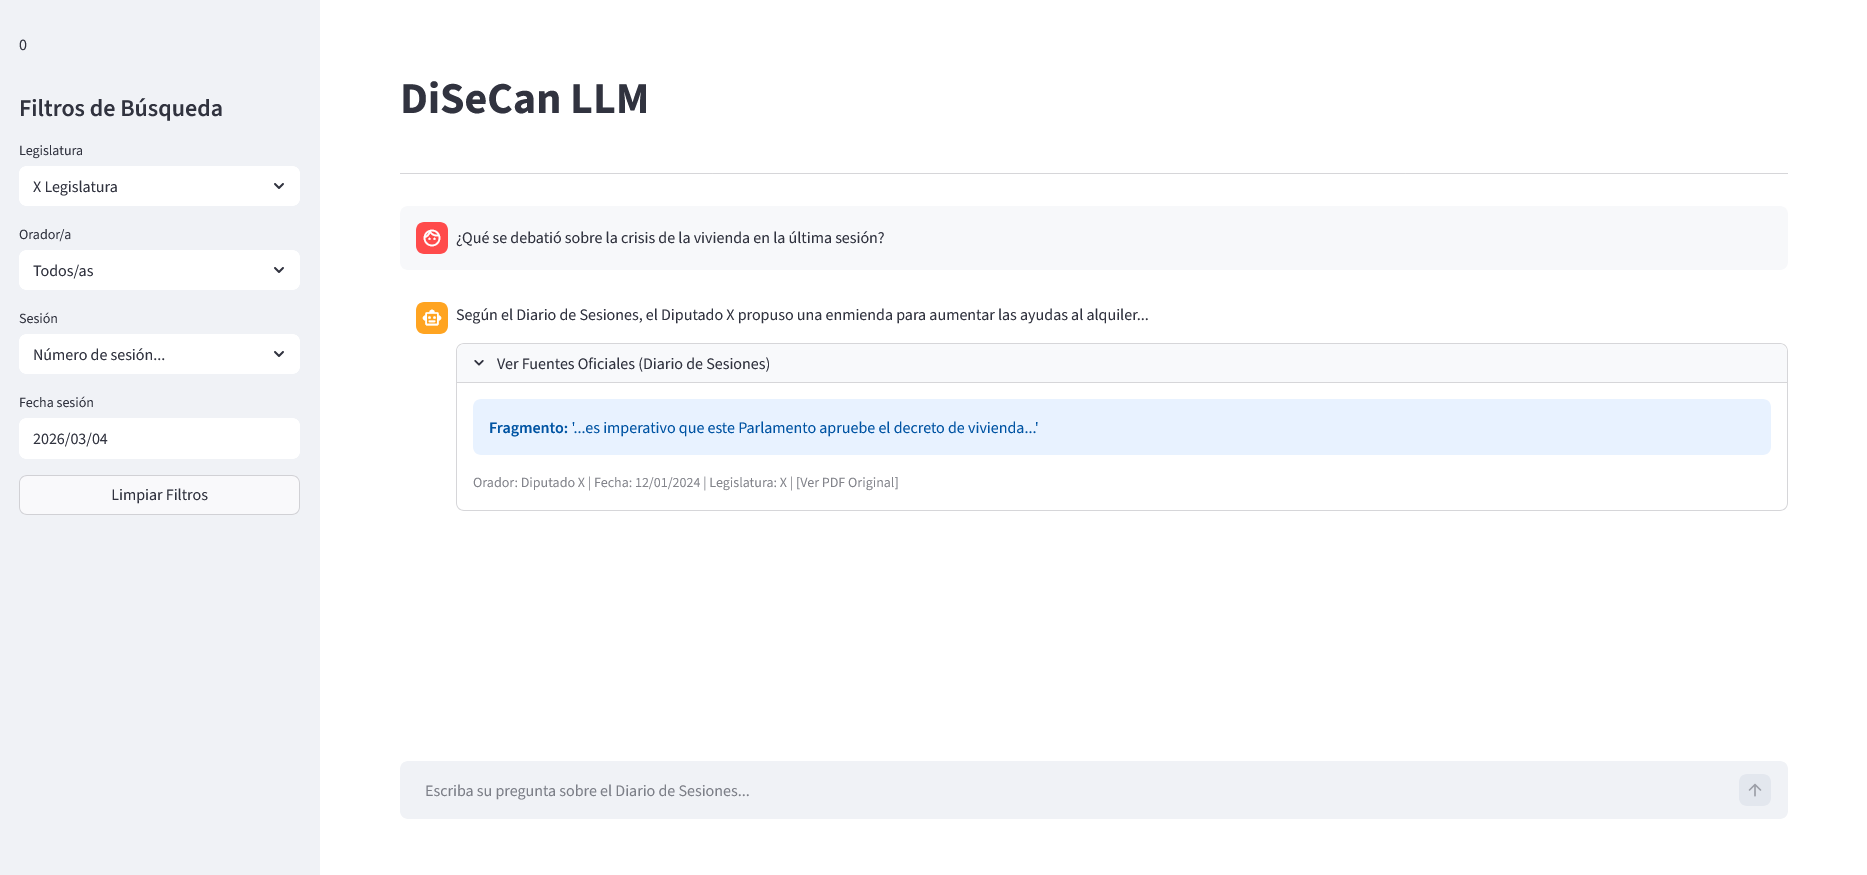
\includegraphics[width=0.8\textwidth]{Ilustraciones/mockuplight.png}
    \caption{Aspecto del sistema en Modo Claro (dispositivo tableta/escritorio).}
    \label{fig:mockuplight}
\end{figure}

\begin{figure}[H]
    \centering
    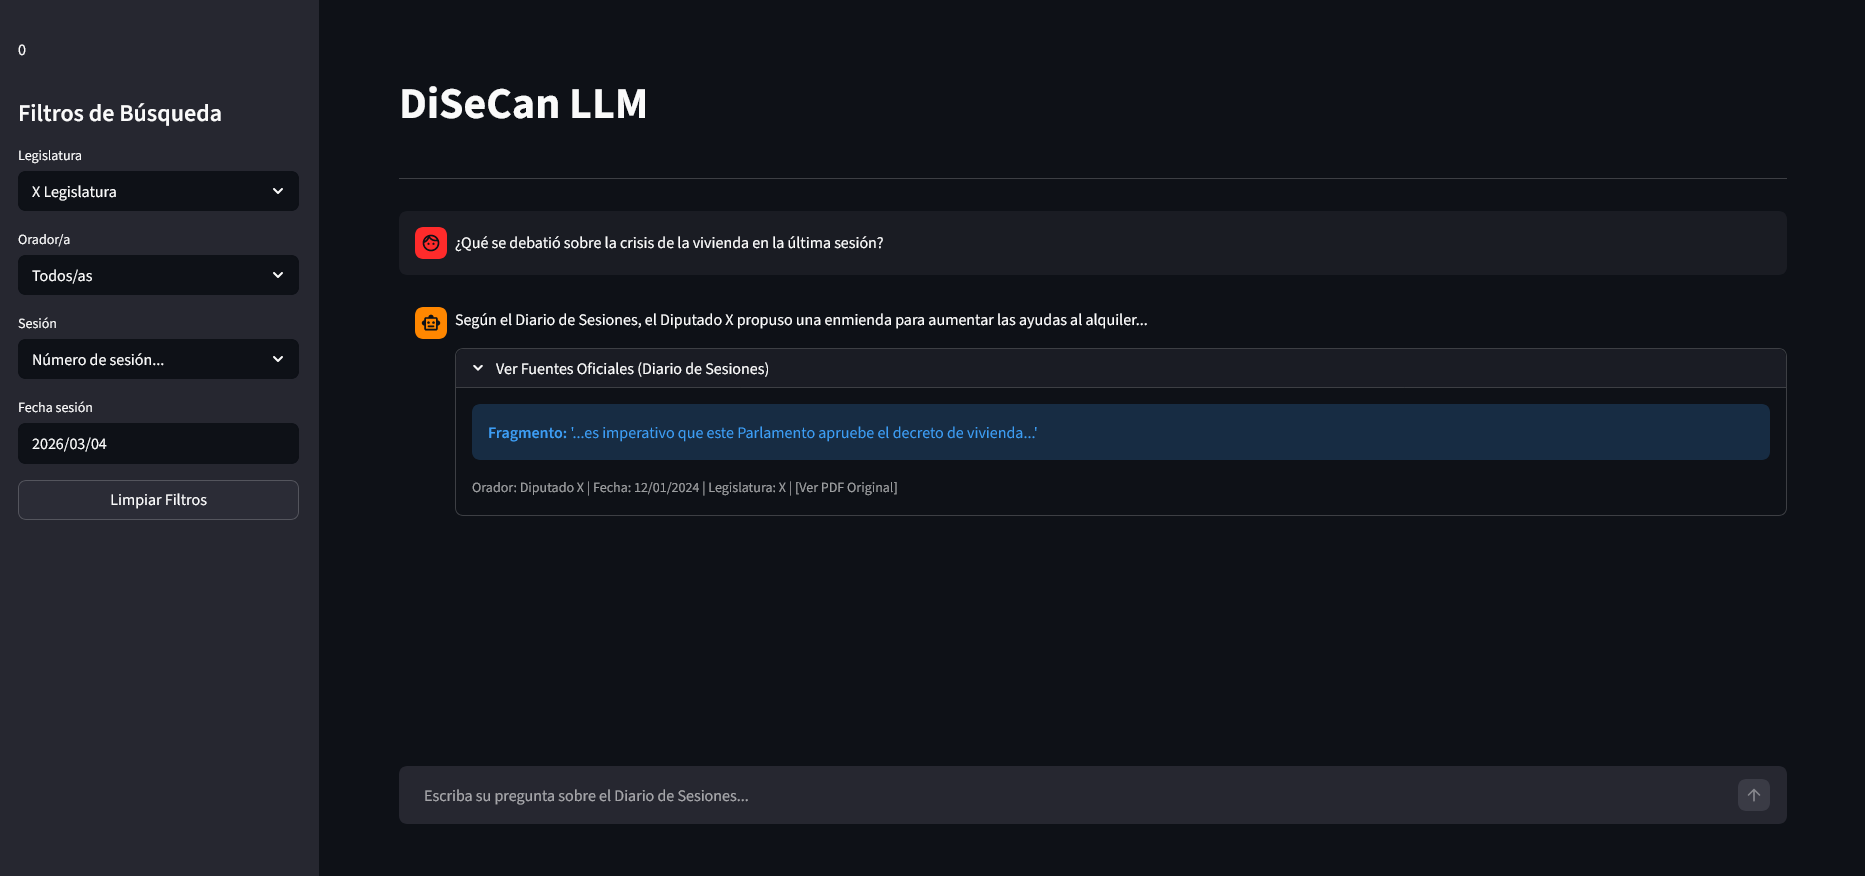
\includegraphics[width=0.8\textwidth]{Ilustraciones/mockupdark.png}
    \caption{Aspecto del sistema en el diseño invertido o Modo Oscuro.}
    \label{fig:mockupdark}
\end{figure}


\chapter{Resultados}
%\input{Resultados.tex}

Presentación de los resultados del trabajo. (Esta sección será desarrollada tras la ejecución de las pruebas experimentales, incluyendo la evaluación de métricas de Faithfulness y Answer Relevancy).

\chapter{Conclusiones y trabajo futuro}
%\input{Conclusiones.tex}

\section{Conclusiones}
El diseño arquitectónico propuesto demuestra que es técnica y logísticamente viable modernizar las herramientas de consulta del Parlamento de Canarias sin comprometer la privacidad de los datos mediante el uso de APIs externas.

\section{Trabajo futuro}
Como vías de extensión, se plantea la transición hacia un paradigma Table-Augmented Generation (TAG), permitiendo al sistema RAG razonar no solo sobre los textos de las intervenciones, sino ejecutar comparativas complejas sobre datos tabulares de votaciones y presupuestos a lo largo de las distintas legislaturas.

\section{Uso de la IA}
En cumplimiento de la normativa académica, se declara que para la ideación de la arquitectura híbrida y la estructuración del código LaTeX de la presente memoria, se ha empleado la asistencia de modelos de lenguaje generativos (Gemini y Claude) operando en entornos como Google Antigravity. Estas herramientas han actuado exclusivamente como soporte a la planificación, siendo el autor humano el responsable íntegro del diseño lógico, validación y ejecución del Trabajo de Fin de Grado.

\chapter{Otros capítulos y anexos}

\section{Normativa y Legislación}
El desarrollo del sistema en modo \textit{on-premise} (servidores locales de la ULPGC) responde directamente a las exigencias del \textbf{Reglamento Europeo de Inteligencia Artificial (AI Act)}. Al tratarse de un sistema orientado a la administración pública y datos institucionales, la arquitectura propuesta asegura la trazabilidad total de las fuentes y previene la fuga de información hacia infraestructuras en la nube de terceros.

\bibliography{ref}
\bibliographystyle{apalike}
\clearpage

\printglossaries

\end{document}